\documentclass[11pt]{article}

% --- Idioma y fuentes ------------------------------------------------
\usepackage[spanish,es-noshorthands,es-tabla]{babel}
\usepackage[T1]{fontenc}
\usepackage{lmodern}

% --- Geometría y encabezado ------------------------------------------
\usepackage[a4paper,margin=2.5cm]{geometry}
\usepackage{fancyhdr}
\setlength{\headheight}{38.22325pt}
\addtolength{\topmargin}{-6.22325pt}

% --- Matemáticas, tablas, figuras -------------------------------------
\usepackage{amsmath,amssymb}
\usepackage[dvipsnames,table]{xcolor}
\usepackage{booktabs}
\usepackage{array}
\usepackage{graphicx}
\usepackage{float}
\usepackage{subcaption}
\usepackage{enumitem}
\usepackage[most]{tcolorbox}
\renewcommand{\arraystretch}{1.3}

% --- BORRADOR: los recuadros rojos dicen qué redactar ------------------
% Para la entrega: cambiar \borradortrue por \borradorfalse (desaparecen).
\newif\ifborrador
\borradortrue
\newcommand{\redactar}[1]{\ifborrador
  \begin{tcolorbox}[colback=red!4,colframe=red!60!black,fonttitle=\bfseries\small,
    title=Redactar (lo escribe el grupo),breakable,left=4pt,right=4pt,top=1pt,bottom=1pt]
  \small #1\end{tcolorbox}\fi}
\newcommand{\grupo}[1]{\ifborrador
  \begin{tcolorbox}[colback=orange!6,colframe=orange!70!black,fonttitle=\bfseries\small,
    title=Para decidir en el grupo (no va en el informe),breakable,left=4pt,right=4pt,top=1pt,bottom=1pt]
  \small #1\end{tcolorbox}\fi}
\newcommand{\cod}[1]{\texttt{\detokenize{#1}}}

\pagestyle{fancy}
\fancyhf{}
\fancyhead[L]{\textbf{Econometría II}\\ Trabajo práctico --- Etapa 2}
\fancyhead[C]{Universidad de Santiago de Chile}
\fancyfoot[C]{\thepage}

\begin{document}
\sloppy

% =====================================================================
%  PORTADA
% =====================================================================
\begin{titlepage}
\centering
\vspace*{3cm}
{\large Universidad de Santiago de Chile}\\[6pt]
{\large Econometría II}\\[2cm]
{\LARGE \textbf{Etapa 2: Análisis univariado y bivariado}}\\[10pt]
{\large Trabajo Práctico --- Admisión Universidad 2026}\\[3cm]

\textbf{Integrantes:}\quad
David Cuevas $\bullet$ Javier Li-Yau $\bullet$ Benjamín Lizana $\bullet$ Ana Nacif

\vspace{0.6cm}

\textbf{Profesor:}\quad Brian Pfeng Ibacache
\qquad
\textbf{Fecha:}\quad 29 de octubre de 2026
\end{titlepage}

% =====================================================================
\section{Introducción}

\redactar{3--5 líneas. Qué se hizo en la Etapa 1 (base y variable de respuesta), qué se corrige ahora (el N, ver §2) y qué busca esta etapa: medir la relación de cada X candidata con $I$ (univariado y bivariado con WOE e IV) para llegar a las X definitivas del logit de la Etapa 3.}

% =====================================================================
\section{Corrección de la base: N = 168.714}

\redactar{Explicar por qué cambia la base. Antes: \cod{full_join} de los cuatro archivos y N = 108.251. Ahora la base maestra es el archivo de rendición (Archivo C), filtrado; las postulaciones (Archivo D) solo dejan una marca, \cod{flag_postula}, y la matrícula (vía 1, tipo 1) se pega con \cod{left_join}. Decir por qué se excluye a quienes ya rindieron antes (evitar sesgo: el profesor lo comparó con excluir a los funcionarios en banca) y por qué los que rindieron y no postularon quedan como $I = 0$.}

\begin{table}[H]
\centering
\caption{Embudo de filtros sobre el archivo de rendición}
\label{tab:embudo}
\begin{tabular}{>{\raggedright}p{8cm} r r}
\toprule
\textbf{Paso} & \textbf{N} & \textbf{Salen} \\
\midrule
Archivo C (rinden la PAES 2026) & 317.700 & --- \\
1. Promoción 2025 (\cod{SITUACION_EGRESO == 1}) & 218.066 & 99.634 \\
2. Rinde por primera vez (sin puntajes de procesos anteriores) & 217.449 & 617 \\
3. Lectora y M1 con puntaje $\geq 100$ & 179.347 & 38.102 \\
4. Ciencias o Historia con puntaje $\geq 100$ & 170.056 & 9.291 \\
5. Promedio de notas distinto de 0 & \textbf{168.714} & 1.342 \\
\bottomrule
\end{tabular}
\end{table}

% =====================================================================
\section{Variable de respuesta}

\redactar{Definir $I$ con palabras y en fórmula: $I = 1$ si el estudiante se matriculó por vía regular (vía 1, tipo 1) en su 1.ª, 2.ª o 3.ª preferencia; $I = 0$ en cualquier otro caso. Comentar la tasa (35,70 \%) y la composición de los ceros (tabla \ref{tab:comp}). Mencionar el chequeo: ningún $I = 1$ tiene \cod{flag_postula = 0}.}

\[
I_i =
\begin{cases}
1 & \text{si } i \text{ se matriculó por vía regular en su preferencia } 1, 2 \text{ o } 3,\\
0 & \text{en otro caso.}
\end{cases}
\]

\begin{table}[H]
\centering
\caption{Composición de la variable de respuesta}
\label{tab:comp}
\begin{tabular}{>{\raggedright}p{9cm} r r}
\toprule
\textbf{Grupo} & \textbf{N} & \textbf{\%} \\
\midrule
$I = 1$: matrícula regular en la preferencia 1, 2 o 3 & 60.234 & 35,70 \\
\midrule
$I = 0$: rindió y no postuló & 54.525 & 32,32 \\
$I = 0$: no postuló y se matriculó por otra vía & 836 & 0,50 \\
$I = 0$: matrícula regular en la preferencia 4 o más abajo & 8.391 & 4,97 \\
$I = 0$: postuló y se matriculó por otra vía o tipo & 6.208 & 3,68 \\
$I = 0$: postuló y no se matriculó & 38.520 & 22,83 \\
\midrule
\textbf{Total} & \textbf{168.714} & \textbf{100,00} \\
\bottomrule
\end{tabular}
\end{table}

% =====================================================================
\section{Análisis univariado}

\redactar{Presentar la tabla \ref{tab:uni}: qué es cada X, de dónde sale (Archivo C, B o Mineduc) y su descriptivo. Dos criterios: (a) con más de 5 \% de NA la variable no se usa: solo falla el ingreso per cápita del grupo familiar (27,66 \%); (b) atípicos según Tukey (tabla \ref{tab:tukey}): se informan pero no se eliminan, porque son casos reales y con el WOE el atípico queda dentro de su tramo. Decir también qué variables se sacaron antes del análisis por ser \emph{ex post} (\cod{PTJE_POND}, \cod{N_MATRICULADOS}).}

\begin{table}[H]
\centering
\small
\caption{Descriptivos de las X candidatas (N = 168.714)}
\label{tab:uni}
\begin{tabular}{>{\raggedright}p{5.6cm} r r r r r}
\toprule
\textbf{Variable} & \textbf{\% NA} & \textbf{Mín.} & \textbf{Mediana} & \textbf{Media} & \textbf{Máx.} \\
\midrule
\multicolumn{6}{l}{\emph{Del estudiante}} \\
Promedio de notas (\cod{PROMEDIO_NOTAS}) & 0 & 4,18 & 6,13 & 6,09 & 7,00 \\
\% superior de notas (\cod{PORC_SUP_NOTAS}) & 0 & 10 & 50 & 47,65 & 100 \\
Puntaje NEM (\cod{PTJE_NEM}) & 0 & 157 & 751 & 737,87 & 1.000 \\
Puntaje ranking (\cod{PTJE_RANKING}) & 0 & 157 & 759 & 750,64 & 1.000 \\
Competencia Lectora (\cod{CLEC_REG_ACTUAL}) & 0 & 100 & 590 & 604,88 & 1.000 \\
Matemática 1 (\cod{MATE1_REG_ACTUAL}) & 0 & 100 & 601 & 628,94 & 1.000 \\
Edad en meses (\cod{EDAD_MESES}) & 0 & 181 & 218 & 222,55 & 860 \\
Ingreso per cápita del grupo familiar (tramo) & \textbf{27,66} & 1 & 4 & 4,78 & 10 \\
Rinde Ciencias (dummy) & 0 & 0 & 1 & 0,72 & 1 \\
Rinde Historia (dummy) & 0 & 0 & 1 & 0,57 & 1 \\
Rinde M2 (dummy) & 0 & 0 & 0 & 0,44 & 1 \\
PACE (dummy) & 0 & 0 & 0 & 0,08 & 1 \\
BEA (dummy) & 0 & 0 & 0 & 0,08 & 1 \\
Sexo, región & 0 & \multicolumn{4}{c}{categóricas} \\
\midrule
\multicolumn{6}{l}{\emph{Del colegio}} \\
Técnico-profesional (dummy) & 0 & 0 & 0 & 0,24 & 1 \\
Dependencia & 0 & \multicolumn{4}{c}{categórica (4 grupos)} \\
N.º de alumnos (\cod{N_ALUMNOS}) & 0 & 8 & 128 & 160,63 & 947 \\
Ingreso del colegio (tramo) & 0,04 & 1 & 4 & 4,55 & 10 \\
\bottomrule
\end{tabular}
\end{table}
\grupo{La edad máxima es 860 meses (71 años). Puede ser real (egresados 2025 de educación de adultos), pero hay que verificarlo y decirlo al comentar los 8.513 atípicos de edad. Revisar también los nombres de las fuentes (Archivo B/C, Mineduc).}

\begin{table}[H]
\centering
\caption{Atípicos según la regla de Tukey ($Q_1 - 1{,}5\,RIC$, $Q_3 + 1{,}5\,RIC$)}
\label{tab:tukey}
\begin{tabular}{l r r r}
\toprule
\textbf{Variable} & \textbf{Límite inf.} & \textbf{Límite sup.} & \textbf{Atípicos} \\
\midrule
Promedio de notas & 4,61 & 7,61 & 61 \\
Puntaje NEM & 316 & 1.172 & 116 \\
Puntaje ranking & 302,5 & 1.210,5 & 77 \\
Competencia Lectora & 215 & 975 & 101 \\
Matemática 1 & 225 & 1.001 & 17 \\
Edad en meses & 204,5 & 232,5 & 8.513 \\
N.º de alumnos & $-93{,}5$ & 374,5 & 8.947 \\
Ingreso del colegio & 0 & 8 & 12.849 \\
\bottomrule
\end{tabular}
\end{table}

% =====================================================================
\section{Análisis bivariado: WOE e IV}

\redactar{(1) Convención: \cod{scorecard} calcula $WOE_j = \ln(\%I_{1,j} / \%I_{0,j})$, así que un WOE positivo indica un tramo con más matrícula en el top 3 que el promedio. (2) Fórmula del IV y escala de Siddiqi (inútil $< 0{,}02$; débil $0{,}02$--$0{,}1$; medio $0{,}1$--$0{,}3$; fuerte $0{,}3$--$0{,}5$; sospechoso $> 0{,}5$). (3) Comentar la tabla \ref{tab:iv}: qué sale por IV $< 0{,}02$ y por qué Lectora y M1 se quedan aunque sean «sospechosas» (el puntaje es la base de la selección, no es una fuga de información). (4) Monotonía: solo edad y N.º de alumnos no lo son.}

\[
WOE_j = \ln\!\left(\frac{\%I_{1,j}}{\%I_{0,j}}\right), \qquad
IV = \sum_j \left(\%I_{1,j} - \%I_{0,j}\right) WOE_j
\]

\begin{table}[H]
\centering
\caption{Valor de información (IV) de las X candidatas, tramos de \cod{woebin}}
\label{tab:iv}
\begin{tabular}{l r c l c l}
\toprule
\textbf{Variable} & \textbf{IV} & \textbf{Tramos} & \textbf{Poder} & \textbf{Monótona} & \textbf{Decisión} \\
\midrule
Competencia Lectora & 0,734 & 5 & sospechoso & sí & sigue \\
Matemática 1 & 0,627 & 5 & sospechoso & sí & sigue \\
Promedio de notas & 0,395 & 5 & fuerte & sí & sigue \\
Puntaje NEM & 0,394 & 5 & fuerte & sí & VIF \\
Puntaje ranking & 0,376 & 5 & fuerte & sí & VIF \\
\% superior de notas & 0,193 & 4 & medio & sí & VIF \\
Técnico-profesional & 0,106 & 2 & medio & sí & sigue \\
Ingreso del colegio & 0,106 & 4 & medio & sí & VIF \\
Dependencia & 0,104 & 4 & medio & sí & agrupar \\
Edad en meses & 0,051 & 3 & débil & \textbf{no} & retramificar \\
Ingreso per cápita & 0,042 & 5 & débil & sí & fuera (NA) \\
BEA & 0,033 & 2 & débil & sí & sigue \\
Rinde M2 & 0,024 & 2 & débil & sí & sigue \\
\midrule
Región & 0,018 & 4 & inútil & sí & fuera \\
Rinde Historia & 0,007 & 2 & inútil & sí & fuera \\
N.º de alumnos & 0,006 & 5 & inútil & \textbf{no} & fuera \\
Rinde Ciencias & 0,002 & 2 & inútil & sí & fuera \\
PACE & 0,001 & 2 & inútil & sí & fuera \\
Sexo & 0,000 & 2 & inútil & sí & fuera \\
\bottomrule
\end{tabular}
\end{table}

\begin{figure}[H]
\centering
\begin{subfigure}{0.48\textwidth}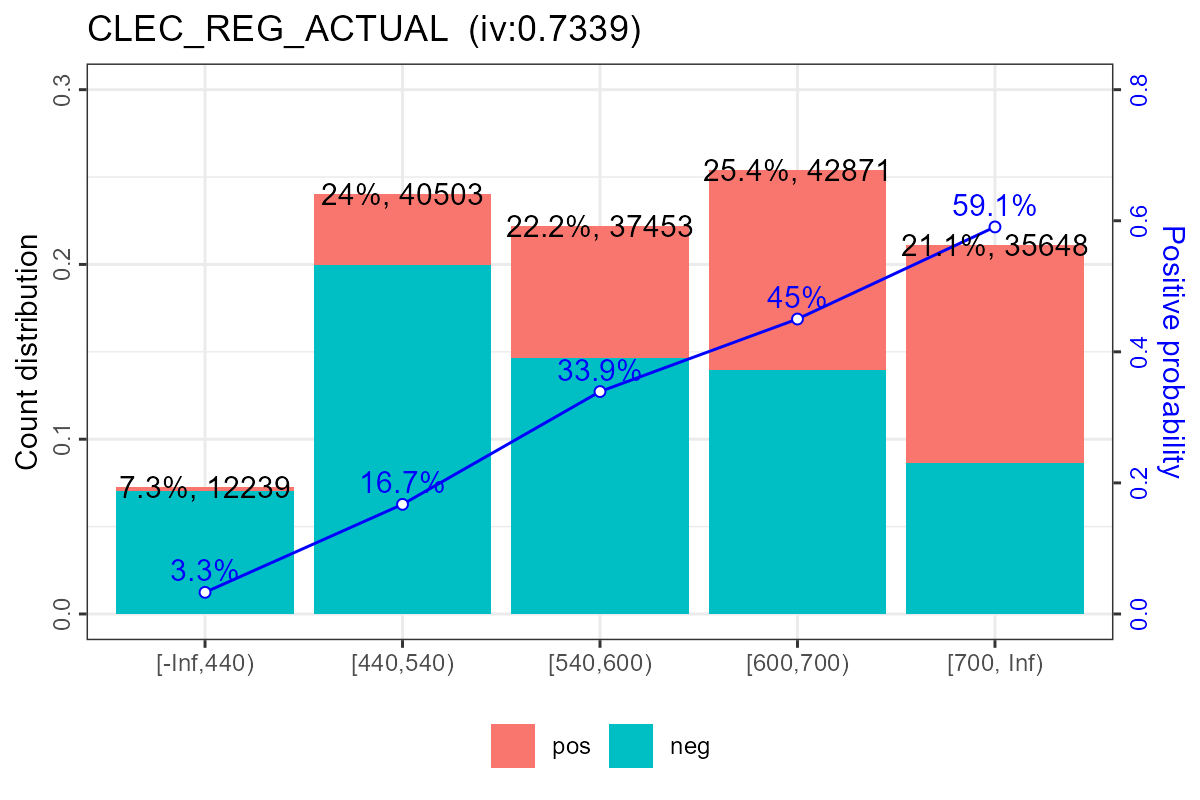
\includegraphics[width=\linewidth]{figuras/woe-CLEC_REG_ACTUAL.png}\end{subfigure}
\hfill
\begin{subfigure}{0.48\textwidth}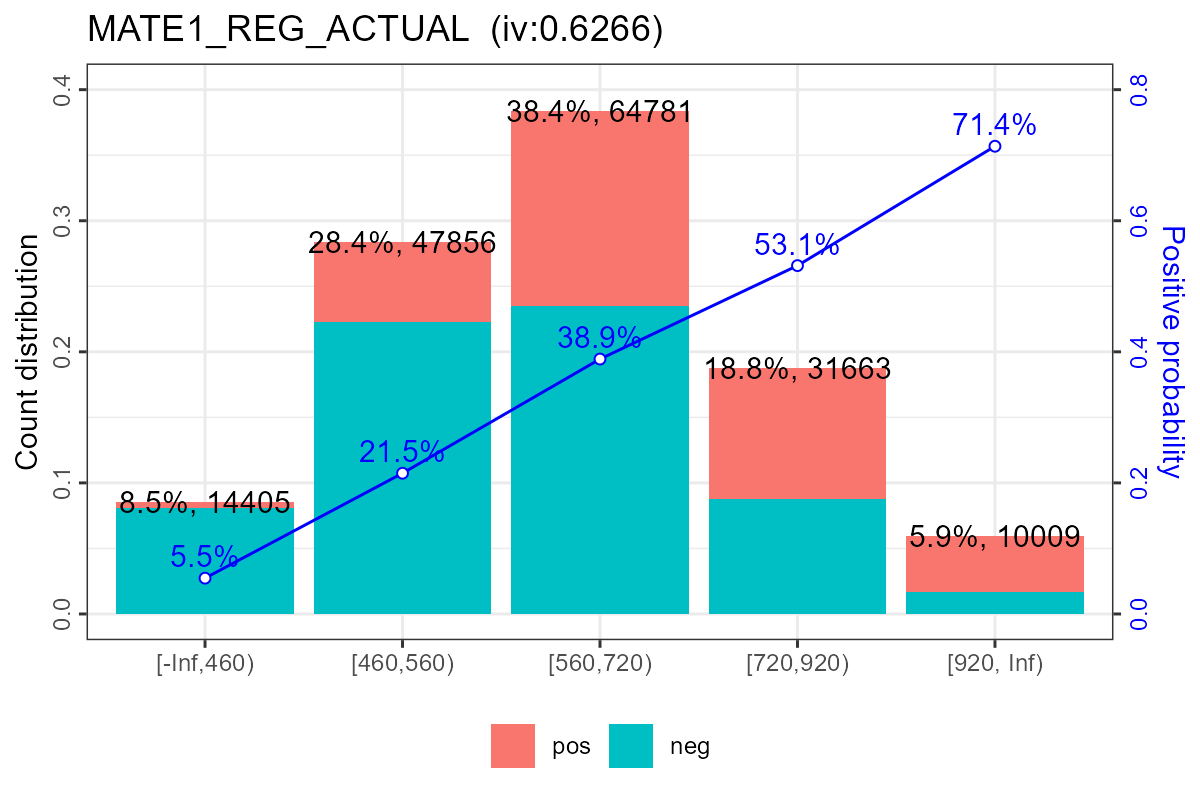
\includegraphics[width=\linewidth]{figuras/woe-MATE1_REG_ACTUAL.png}\end{subfigure}\\[4pt]
\begin{subfigure}{0.48\textwidth}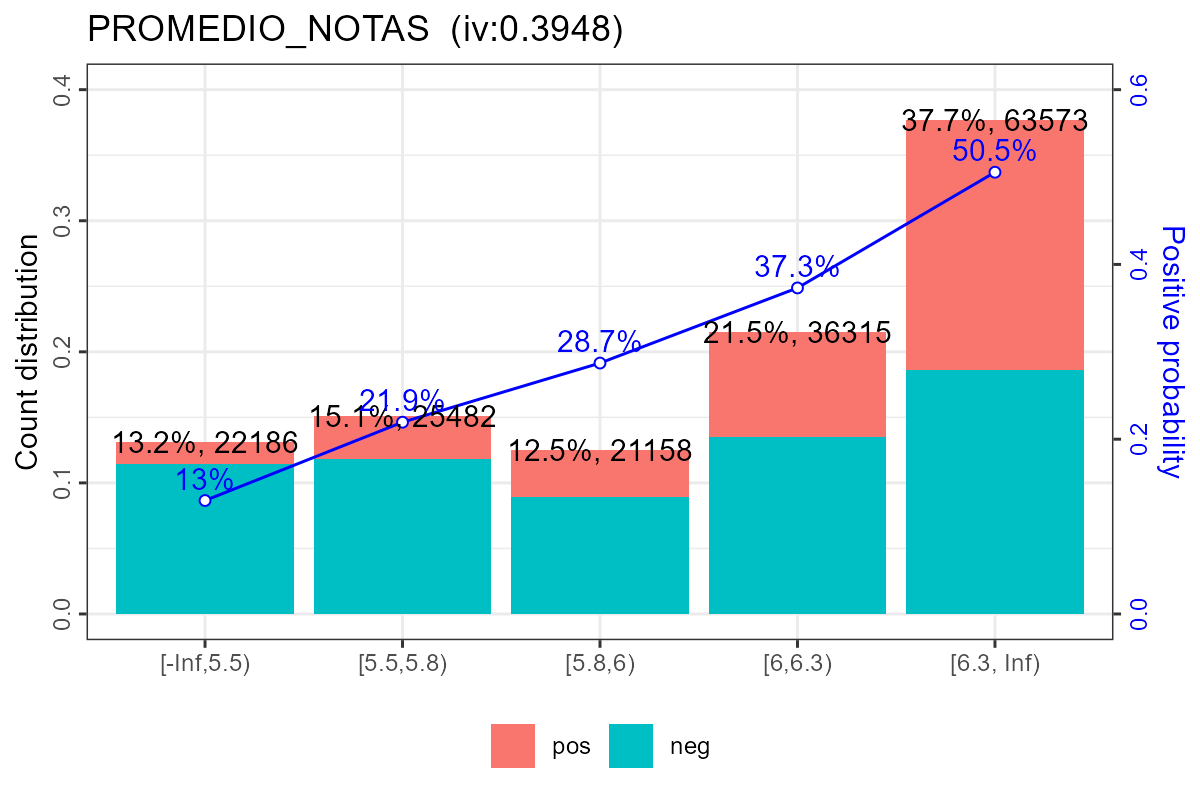
\includegraphics[width=\linewidth]{figuras/woe-PROMEDIO_NOTAS.png}\end{subfigure}
\hfill
\begin{subfigure}{0.48\textwidth}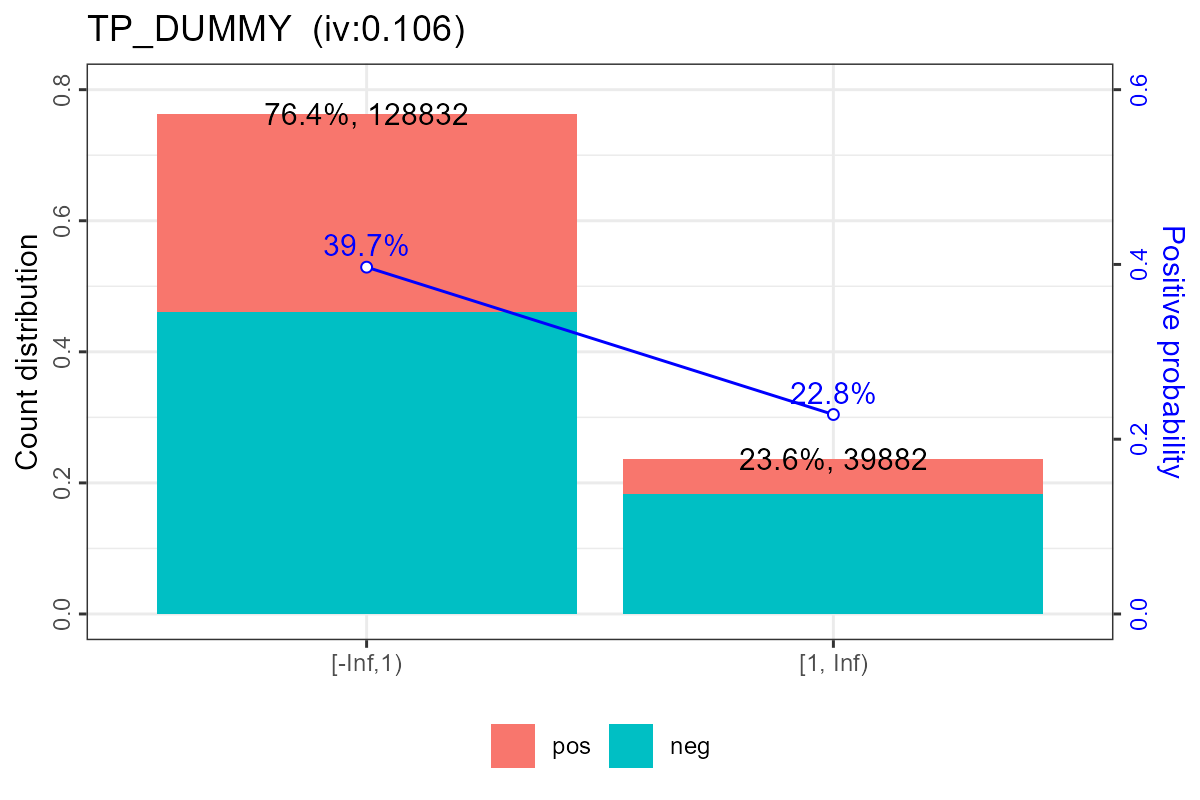
\includegraphics[width=\linewidth]{figuras/woe-TP_DUMMY.png}\end{subfigure}
\caption{Peso de cada tramo (barras) y tasa de $I = 1$ (línea) de las X con mayor IV}
\label{fig:woe}
\end{figure}

\redactar{Leer la figura \ref{fig:woe} en 2--3 líneas: la tasa de matrícula en el top 3 sube de forma monótona con Lectora (3,3 \% a 59,1 \%), M1 (5,5 \% a 71,4 \%) y el promedio de notas (13,0 \% a 50,6 \%); en los colegios técnico-profesionales es 22,8 \% contra 39,7 \%.}

% =====================================================================
\section{Retramificación}

\redactar{Por qué se exige monotonía (el WOE debe ir de negativo a positivo para que el logit lo lea con un solo signo) y que cada tramo pese al menos 5 \%. Edad: \cod{woebin} cortó en 216 y 228 meses y la tasa sube y luego baja (35,5 | 38,1 | 20,6 \%); con un solo corte en 228 meses (19 años) queda monótona, con IV 0,049 y un segundo tramo de 9 \%. Dependencia: por juicio experto se juntan municipal y SLEP como «público». Decir qué se pierde de IV al retramificar (casi nada).}

\begin{table}[H]
\centering
\caption{Tramos después de retramificar}
\label{tab:retr}
\begin{tabular}{l l r r r}
\toprule
\textbf{Variable} & \textbf{Tramo} & \textbf{Peso} & \textbf{Tasa $I = 1$} & \textbf{WOE} \\
\midrule
Edad en meses (IV 0,049) & menos de 228 & 91,0 \% & 37,2 \% & 0,064 \\
                         & 228 o más     & 9,0 \%  & 20,6 \% & $-0{,}761$ \\
\midrule
Dependencia (IV 0,104) & público (municipal y SLEP) & 34,0 \% & 28,6 \% & $-0{,}325$ \\
                       & particular subvencionado & 53,1 \% & 36,0 \% & 0,012 \\
                       & particular pagado & 12,9 \% & 53,1 \% & 0,712 \\
\bottomrule
\end{tabular}
\end{table}

\begin{figure}[H]
\centering
\begin{subfigure}{0.48\textwidth}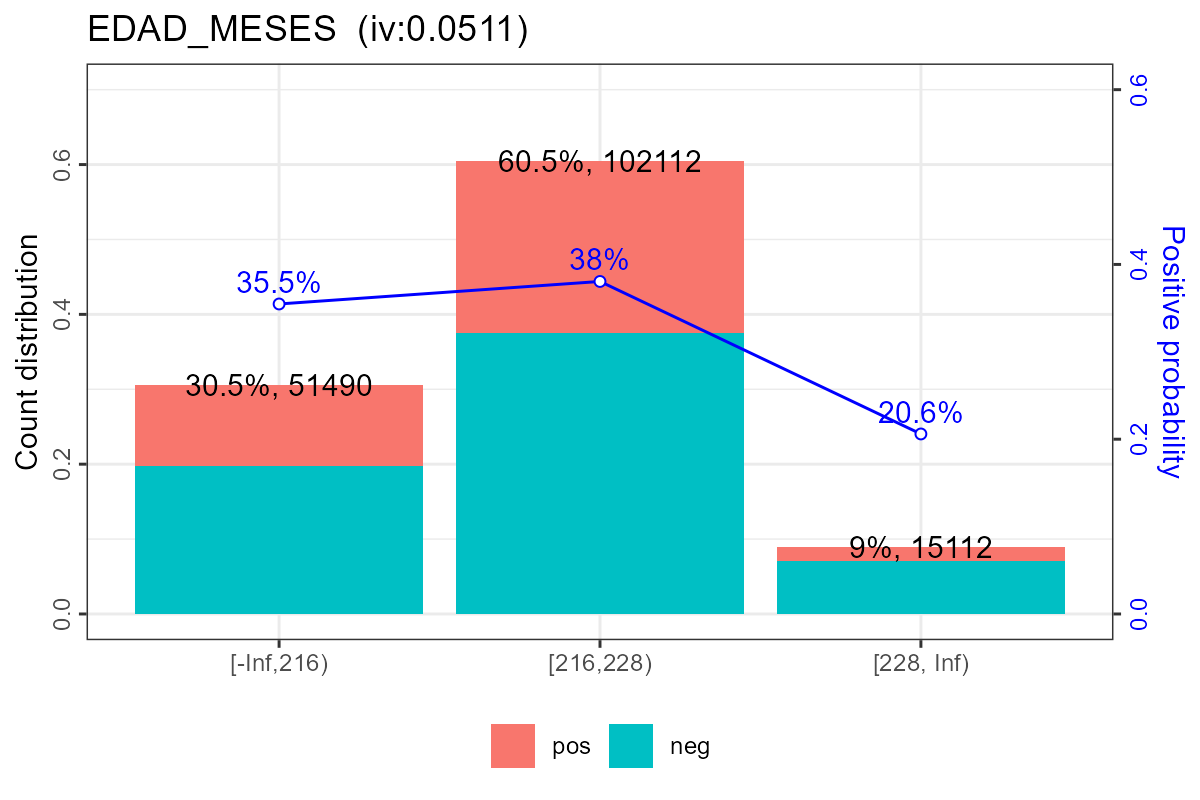
\includegraphics[width=\linewidth]{figuras/edad-antes.png}\caption{Edad: antes}\end{subfigure}
\hfill
\begin{subfigure}{0.48\textwidth}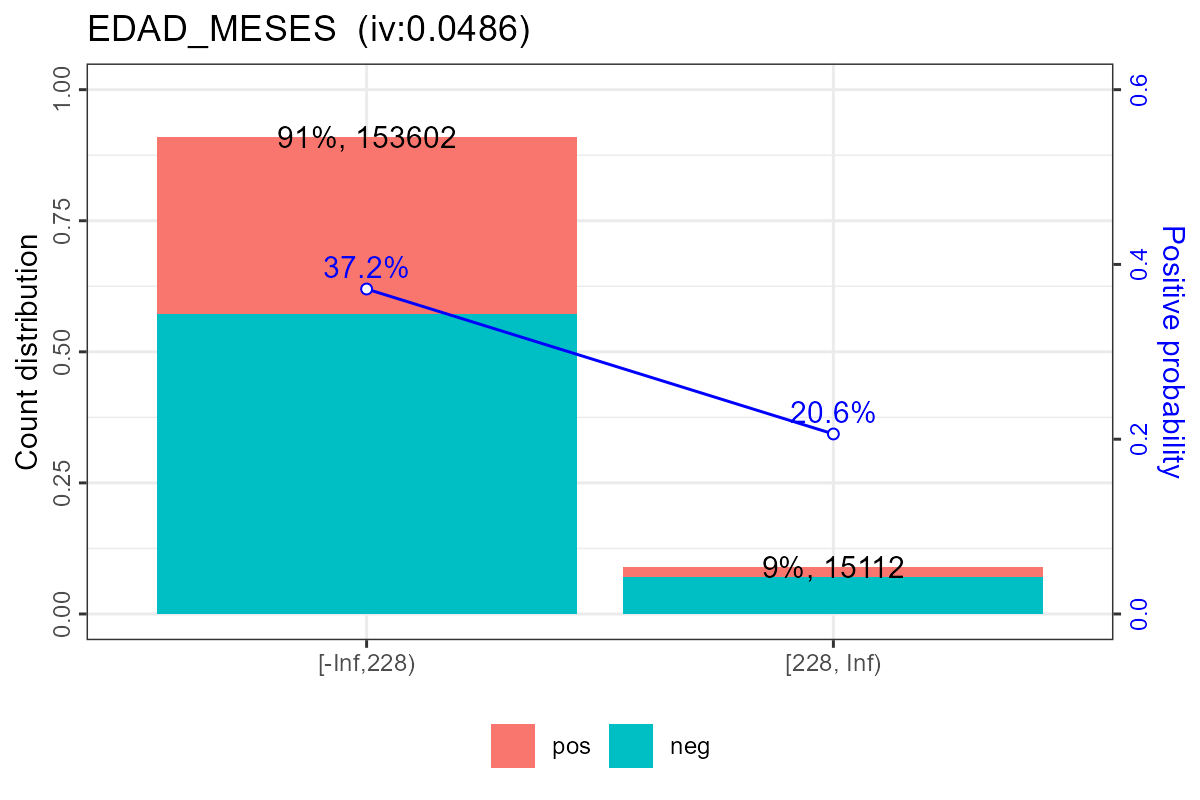
\includegraphics[width=\linewidth]{figuras/edad-despues.png}\caption{Edad: después}\end{subfigure}\\[4pt]
\begin{subfigure}{0.48\textwidth}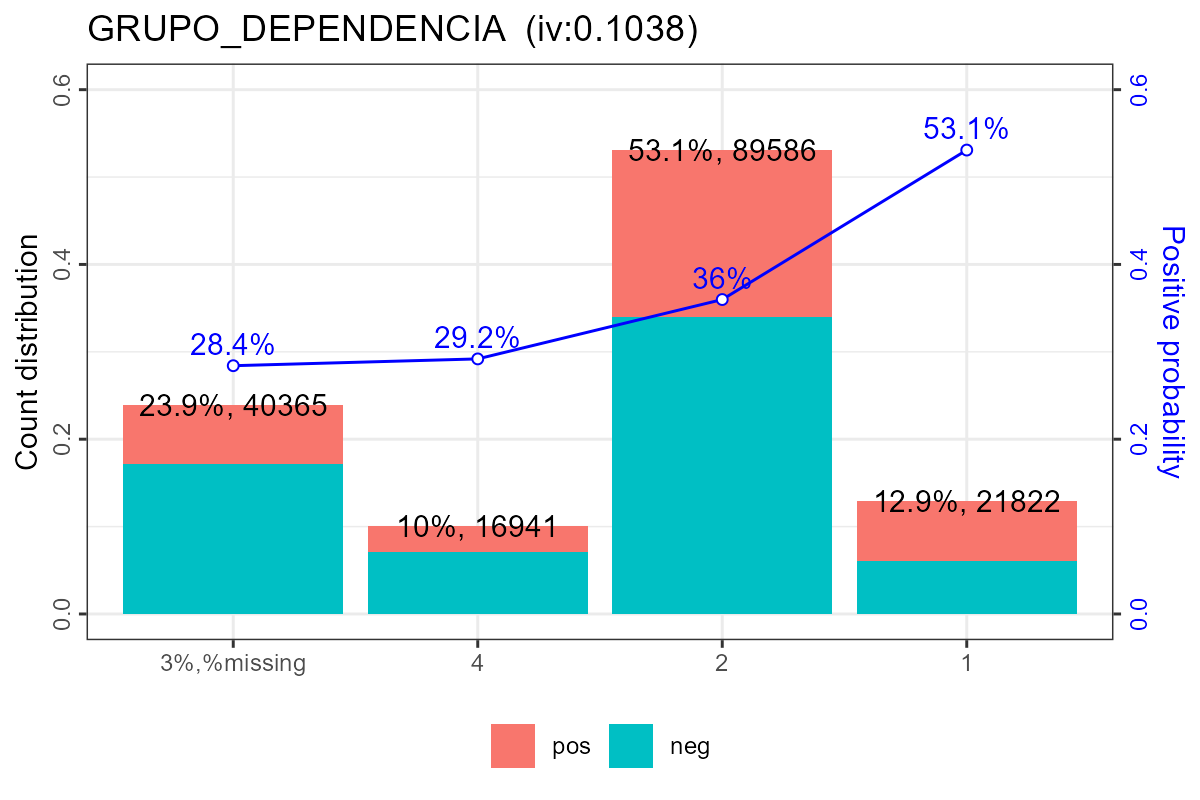
\includegraphics[width=\linewidth]{figuras/dependencia-antes.png}\caption{Dependencia: antes}\end{subfigure}
\hfill
\begin{subfigure}{0.48\textwidth}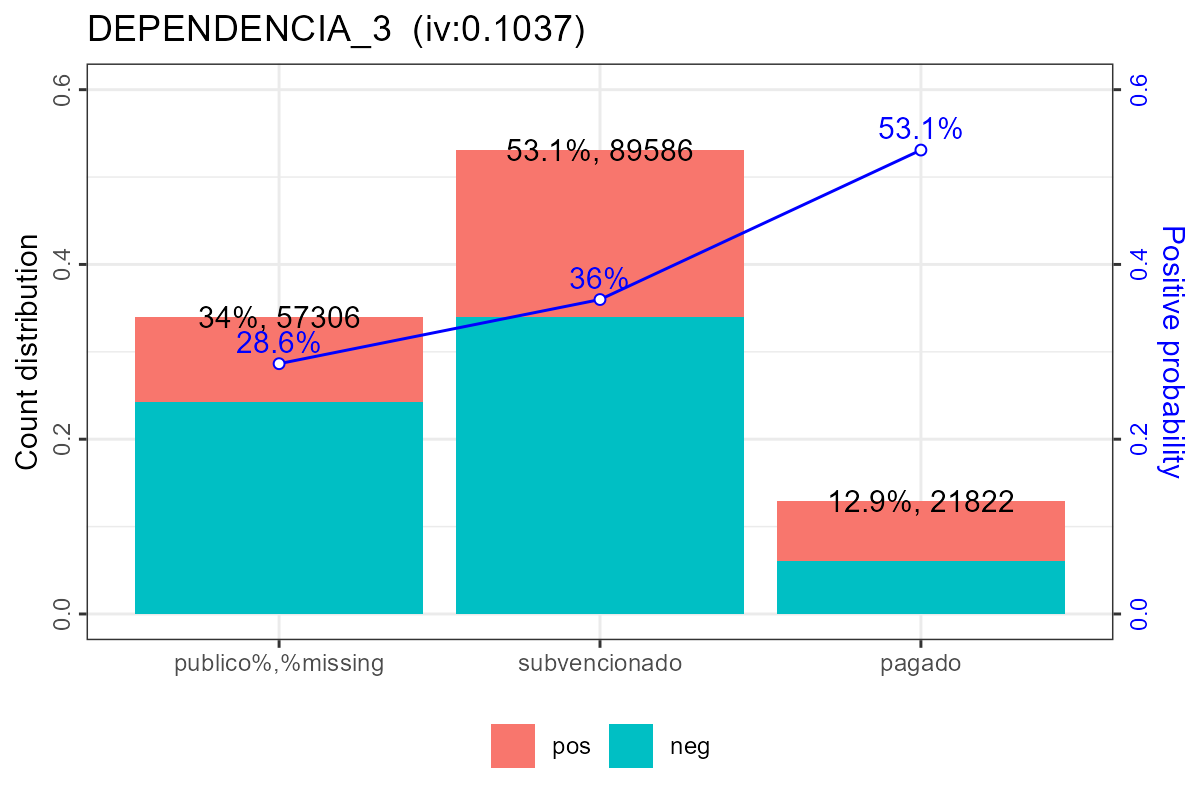
\includegraphics[width=\linewidth]{figuras/dependencia-despues.png}\caption{Dependencia: después}\end{subfigure}
\caption{Retramificación de edad y dependencia}
\label{fig:retr}
\end{figure}

\grupo{En «dependencia antes», \cod{woebin} juntó solo el grupo municipal con los NA (\cod{3\%,\%missing}), y en «después» los NA quedan dentro de «público». Son muy pocos, pero hay que decir dónde quedaron. Revisar también los códigos de \cod{GRUPO_DEPENDENCIA} (1 pagado, 2 subvencionado, 3 municipal, 4 SLEP) contra el libro de códigos.}

% =====================================================================
\section{X definitivas y multicolinealidad}

\redactar{Explicar el VIF sobre la base «woeizada» (cada X reemplazada por el WOE de su tramo), con el umbral que dio el profesor (VIF $> 2$, sale). Con las 12 que pasan el IV, NEM, ranking y promedio se pisan (VIF de 12,8 a 17,8): queda el promedio, que tiene el mayor IV. Sale el \% superior (VIF 3,4). Entre dependencia e ingreso del colegio (VIF 2,4 y 2,3) se deja una. Con las 8 finales todas quedan bajo 2. Cerrar con la tabla de signos esperados (tabla \ref{tab:signo}) justificados con juicio experto: esto lo destacó el profesor en la Etapa 1.}

\begin{table}[H]
\centering
\caption{VIF con las 12 X que pasan el IV y con las 8 definitivas}
\label{tab:vif}
\begin{tabular}{l r r}
\toprule
\textbf{Variable (WOE)} & \textbf{VIF, 12 X} & \textbf{VIF, 8 X} \\
\midrule
Competencia Lectora & 1,60 & 1,59 \\
Matemática 1 & 1,76 & 1,73 \\
Promedio de notas & 12,82 & 1,31 \\
Puntaje NEM & 17,76 & --- \\
Puntaje ranking & 15,20 & --- \\
\% superior de notas & 3,37 & --- \\
Técnico-profesional & 1,18 & 1,14 \\
Ingreso del colegio & 2,34 & --- \\
Dependencia (3 tramos) & 2,38 & 1,25 \\
Edad (2 tramos) & 1,04 & 1,04 \\
BEA & 1,19 & 1,14 \\
Rinde M2 & 1,11 & 1,11 \\
\bottomrule
\end{tabular}
\end{table}

\begin{table}[H]
\centering
\caption{X definitivas y signo esperado}
\label{tab:signo}
\begin{tabular}{>{\raggedright}p{3.6cm} >{\raggedright}p{2.6cm} c >{\raggedright\arraybackslash}p{4.8cm}}
\toprule
\textbf{X} & \textbf{Tramos} & \textbf{Signo} & \textbf{Por qué} \\
\midrule
Competencia Lectora & 5, creciente & $+$ & \emph{(redactar)} \\
Matemática 1 & 5, creciente & $+$ & \emph{(redactar)} \\
Promedio de notas & 5, creciente & $+$ & \emph{(redactar)} \\
Técnico-profesional & 2 & $-$ & \emph{(redactar)} \\
Dependencia & 3 & $+$ hacia pagado & \emph{(redactar)} \\
Edad & 2 (corte en 19 años) & $-$ & \emph{(redactar)} \\
BEA & 2 & $+$ & \emph{(redactar)} \\
Rinde M2 & 2 & $+$ & \emph{(redactar)} \\
\bottomrule
\end{tabular}
\end{table}

\grupo{\textbf{Ojo con los signos del glm sobre WOE} (sale en el mismo VIF del script). Con WOE todos los $\beta$ deberían ser positivos, y por esa regla se sacó el \% superior ($\beta = -0{,}13$). Pero con las 8 finales también salen negativos y no significativos: dependencia ($\beta = -0{,}011$, $p = 0{,}55$), BEA ($-0{,}003$, $p = 0{,}92$) y Rinde M2 ($-0{,}063$, $p = 0{,}10$). Con las 12, el ingreso del colegio sí sale positivo ($0{,}033$) y la dependencia negativa. Opciones: (a) aplicar la misma regla y dejarlas para la Etapa 3 con aviso; (b) cambiar dependencia por ingreso del colegio; (c) no mencionar signos del glm en esta etapa (el profesor pidió el VIF como avance). Hay que decidirlo antes del jueves, porque el profesor puede preguntar.}

% =====================================================================
\section{Conclusión y próximos pasos}

\redactar{3--4 líneas: de 19 X candidatas quedan 8; las más predictivas son los puntajes PAES y las notas; el colegio (dependencia, TP) aporta información media. En la Etapa 3 se estimará el logit con estas X (tres modelos alternativos) y se interpretarán los efectos.}

\end{document}
